
%(BEGIN_QUESTION)
% Copyright 2011, Tony R. Kuphaldt, released under the Creative Commons Attribution License (v 1.0)
% This means you may do almost anything with this work of mine, so long as you give me proper credit

Calculate the line-of-sight distance between these {\sl Wireless}HART instruments, based on locations shown on this plot plan of an industrial processing unit.  Each division on the map is equivalent to a distance of 5 feet:

$$\includegraphics[width=15.5cm]{i00930x01.eps}$$

\begin{itemize}
\item{} Distance from Gateway to FT-34 = 
\vskip 10pt
\item{} Distance from TT-10 to FT-34 = 
\vskip 10pt
\item{} Distance from Gateway to LT-13 = 
\vskip 10pt
\item{} Distance from TT-10 to AT-77 = 
\end{itemize}

\vfil 

\underbar{file i00930}
\eject
%(END_QUESTION)





%(BEGIN_ANSWER)

This is a graded question -- no answers or hints given!

%(END_ANSWER)





%(BEGIN_NOTES)

Each line-of-sight distance is simply a trigonometric calculation (the Pythagorean Theorem, whereby the length of the hypotenuse of a right triangle is equal to the square-root of the sum of the squares of the side lengths).  Note that each square on the grid is 5 feet in height and width:

\begin{itemize}
\item{} Distance from Gateway to FT-34 = {\bf 60.1 feet} 
\item{} Distance from TT-10 to FT-34 = {\bf 104.7 feet} 
\item{} Distance from Gateway to LT-13 = {\bf 77.6 feet} 
\item{} Distance from TT-10 to AT-77 = {\bf 55 feet}
\end{itemize}

%INDEX% Mathematics review: trigonometric calculations

%(END_NOTES)


